\chapter{Einführung} % (fold)
\label{cha:einführung}

\emph{„How people work is one of the best kept secrets in America.“} (Wellman, D. zitiert nach \cite{Suchman95}).

Diese Aussage David Wellmans diente Lucy Suchman in den 90er-Jahren des 20. Jahrhunderts als Motivator für ihre Forschung über die Natur menschlicher Arbeit im Computerzeitalter und deren Unterstützung durch neue Technologien. Ihre Arbeiten und viele andere (etwa \cite{Schmidt92} oder \cite{Sachs95}) argumentieren für eine stärkere Berücksichtigung der Rolle des Menschen im Arbeitsprozess.

Wellman spielt mit diesem Zitat auf die oft auftretende Diskrepanz zwischen der (niedergeschriebenen) Definition eines Arbeitsablaufs und dessen tatsächlicher Umsetzung in der konkreten betrieblichen Umgebung an.

Der Druck in der heutigen Geschäftswelt, bestimmte Qualitätskriterien garantiert erfüllen zu können, hat zu einer beinahe flächendeckenden Verbreitung von Qualitätszertifizierungen geführt. Die bekanntesten Vertreter dieser Zertifizierungen sind wohl die Standards aus der Familie der ISO 9000 Normen \cite{ISO05}. In der ISO 9001-Norm \cite{ISO00}, in der die Anforderungen an Qualitätsmanagement-Systeme definiert sind, ist festgeschrieben, dass eine prozessorientierte Organisation eine der Voraussetzungen für erfolgreiches Qualitätsmanagement ist. Ein wesentliches Merkmal einer prozessorientierten Organisation ist, dass ihre organisationalen Prozesse — also ihre Arbeitsorganisation und -abläufe — bekannt, benannt und definiert sind. 

Die Unterschiede zwischen festgeschriebenen und gelebten Arbeitsabläufen wurde schon 1978 von Argyris und Schön \cite{Argyris78} beschrieben. Mit der Unterscheidung zwischen „\emph{espoused theories}“ (= \emph{die offiziell veröffentlichten Theorien über Arbeit}) und den „\emph{theories-in-use}“ (= \emph{die tatsächlich handlungsleitenden Theorien}) wurden dieser Gegensatz auch explizit benannt. Sachs \cite{Sachs95} beschreibt das gleiche Phänomen und unterscheidet zwischen dem „\emph{explicit organisational view}“ und dem „\emph{tacit organisational view}“ auf Arbeit. Sie beschreibt damit einerseits eine explizit formulierte und statische Sicht auf Arbeit und andererseits eine informelle, im Fluss befindliche und zum Zeitpunkt der Betrachtung nirgendwo niedergeschriebene Sicht auf Arbeit. Letztere kann lediglich aus der Analyse der tatsächlichen Arbeitsabläufe gewonnen werden kann, die den Tätigkeiten zugrunde liegenden Annahmen („theories-in-use“ \cite{Argyris78}) sowie deren vom Arbeitenden konkret wahrgenommene organisationale Rahmenbedingungen bleiben allerdings verborgen — die Frage nach dem „Warum?“, die die Form des konkreten Arbeitsablaufs motiviert, kann nicht unmittelbar beantwortet werden.

Wie Sachs verdeutlichen auch Wellman sowie Argyris und Schön, dass das zweitgenannte Verständnis von Arbeit nicht explizit niedergeschrieben und formal definiert ist — in seinem Wesen also „unbekannt“ ist. Wenn „Arbeit“ oder die ihr zugrunde liegenden Annahmen unbekannt sind, kann eine Veränderung ihrer selbst oder der Umgebung, in der sie durchgeführt wird, zu schwerwiegenden Problemen führen (wie z.B. von \cite{Nonaka95}, \cite{Krogh00} oder \cite{Gerson86} beschrieben). Der Begriff „Veränderung“ deckt dabei nicht nur tiefgreifende organisatorische Änderungen im Unternehmen ab, sondern durchaus auch „marginale“ Änderungen wie z.B. die Einstellung neuer Mitarbeiter oder dem Einsatz eines neuen Werkzeugs \cite{Olesen03}. Daraus kann man schließen, dass potentiell „problematische“ Situationen häufig auftreten können. 

„Problematische“ Situationen sind dabei all jene Situationen, in denen die Zielerreichung erschwert wird, weil die dazu notwendigen Schritte entweder unklar sind oder nicht operationalisiert werden können. Im Kontext der obigen Aussage bedeutet dies, dass durch eine organisationale Veränderung neue Arbeitsschritte notwendig werden bzw. die bisherigen nicht mehr funktionieren oder angemessen sind. Beim Auftreten einer derartigen Veränderung ist daher eine erneute Planung bzw. Abstimmung der zur Zielerreichung notwendigen Arbeitsschritte notwendig. Fujimura \cite{Fujimura87} unterscheidet in diesem Sinne zwischen zwei Formen von Arbeit — der „Produktion“ („\emph{production}“) und der „Artikulation“ („\emph{articulation}“), wobei letztere alle Tätigkeiten umfasst, die die Umsetzung bzw. Aufrechterhaltung der „Produktion“ ermöglichen.

„Artikulation“ ist ein integraler Bestandteil von Arbeit \cite{Strauss85}. Mit der Komplexität der „Produktion“ steigt auch der Aufwand der dazu notwendigen „Artikulation“ an \cite{Strauss88}. Die Komplexität steigt hier mit der Anzahl der benötigten Arbeitsschritte, den dazu benötigten Kompetenzen und der Anzahl der involvierten Personen. Nicht bekannte, falsche oder zurückgehaltene Information über die „Produktion“ erschweren die „Artikulation“ oder machen sie unmöglich \cite{Fujimura87}. Dies hat jedoch nicht nur negative Auswirkungen auf die „Produktion“ sondern verhindert auch eine tiefergehende Beschäftigung mit der aktuellen Arbeitspraxis und eine potentielle Verbesserung derselben \cite{Argyris78}. Erfolgreiche Artikulation ist damit nicht nur eine Voraussetzung für eine funktionierende Produktion sondern auch ein Enabler für organisationale Veränderungen im Sinne eines organisationalen Lernprozesses (z.B. \cite{Kim93} oder \cite{Firestone03a}).

Eine methodische und technische Unterstützung kann Artikulation ermöglichen oder deren erfolgreichen Ablauf erleichtern (\cite{Schmidt92}, \cite{Simone99}, \cite{Jorgensen04}, \cite{Baker07}).

\fbox{\parbox{13cm}{\textbf{In der Arbeit sind die methodischen und technischen Möglichkeiten zur Ermöglichung und Unterstützung von Articulation Work zu ergründen, die gewonnenen Erkenntnissen in einem Werkzeug umzusetzen und dessen Auswirkungen auf die Interaktion zur Verbesserung der Production Work zu bewerten.}}}

\section{Forschungsfragen} % (fold)
\label{sec:forschungsfragen}

\begin{enumerate}
	\item Wie kann Articulation Work ermöglicht und unterstützt werden?
		\begin{enumerate}
			\item Durch welche Aktivitäten zeigt sich Articulation Work im Arbeitsprozess?
			\item Welche Rahmenbedingungen ermöglichen bzw. begünstigen Articulation Work?
			\item Wie können die in 1.1. identifizierten Aktivitäten unterstützt werden?
			\item Wie können die in 1.2. identifizierten Rahmenbedingungen und die in 1.3. identifizierten Anforderungen in einer Methodik umgesetzt werden?
		\end{enumerate}
	\item Was muss ein Werkzeug zur Unterstützung von Articulation Work leisten?
		\begin{enumerate}
			\item Welche Anforderungen an ein Werkzeug ergeben sich aus der in 1.4. entwickelten Methodik?
			\item Wie können diese Anforderungen technologisch umgesetzt werden?
		\end{enumerate}
	\item Inwiefern unterstützt das entwickelte Werkzeug die Durchführung von Articulation Work?
		\begin{enumerate}
			\item Wie kann die Unterstützungsleistung bewertet werden?
			\item Welche Auswirkungen auf die Interaktion hat die Anwendung von Methodik und Werkzeug?
		\end{enumerate}
\end{enumerate}

% section forschungsfragen (end)

\section{Anmerkung zur wissenschaftstheoretischen Grundlage}

Dieser Arbeit basiert auf den Annahmen des Konstruktivismus. Die Grundannahme, auf der die weiteren Ausführungen basieren, ist die Exisitenz von individuellen "Realitäten", die aufgrund der Wahrnehmung eines Indivuduums, seiner Erfahrungen und Grundannahmen der Welt gebildet wird. Die Existenz einer objektiv exitierenden "Realität" wird angenommen (aber nicht paradigmatisch vorausgesetzt). Die individuellen "Realitäten" stehen insofern in Zusammenhang mit einer objektiven "Realität", als dass letztgenannte -- gefiltert durch Wahrnehmung, Erfahrungen und Grundannahmen -- die Grundlage der erstgenannten bildet.

Ziel dieser Arbeit ist es aus dieser Perspektive, individuelle Realitäten abzustimmen, also die filternden Faktoren individuell so zu beeinflussen, dass die für eine Zusammenarbeiten relevanten Bereiche der objektiven "Realität" zu ähnlichen Abbildungen in der individuellen "Realität" führen.

% chapter einführung (end)
\section{Aufbau der Arbeit} % (fold)
\label{sec:aufbau_der_arbeit}

\subsection{Überblick} % (fold)
\label{sub:aufbau_ueberblick}

Die Arbeit gliedert sich inhaltlich in drei große Teile, die vom Einleitungs- und Schlusskapitel eingerahmt werden.

Teil \ref{prt:grundlagen} behandelt die konzeptuellen Grundlagen der Arbeit und schafft die Argumentationsgrundlage für die Entwicklung des Werkzeugs. Im Einzelnen umfasst Teil \ref{prt:grundlagen} ein Kapitel über Articulation Work (Kapitel \ref{cha:articulation_work}) und eines über Mentale Modelle (Kapitel \ref{cha:mentale_modelle}). Teil \ref{prt:grundlagen} endet mit einem Kapitel über Methodik der Anwendungsszenarien, in dem beschrieben wird, wie Mentale Modelle für die Verwendung für Articulation Work externalisiert und abgestimmt werden können (Kapitel \ref{cha:methodik}).

Teil \ref{prt:umsetzung} behandelt die Umsetzung des Werkzeugs selbst. Das erste Kapitel greift die Ergebnisse des ersten Teils auf und leitet daraus die Anforderungen an das Werkzeug ab (Kapitel \ref{cha:anforderungen}). In Kapitel \ref{cha:implementierung_Überblick} werden die konzeptuellen Grundlagen für die Implementierung aus dem Kontext von Tangible Interfaces heraus aufgearbeitet. Die Kapitel \ref{cha:input_&_interpretation}, \ref{cha:visualisierung} und \ref{cha:persistierung} beschreiben nacheinander die technische Umsetzung des Werkzeugs -- beginnend von den Eingabekanälen über die Ausgabekanäle bis zu Persistierung der Modelle. 

Teil \ref{prt:evaluierung} behandelt die Evaluierung des Werkzeugs. Dabei beginnt Kapitel \ref{cha:konzeptionelle_evaluierung} mit einer konzeptuellen Betrachtung des umgesetzten Systems (also einer theoretischen Einordnung des Werkzeugs auf Basis der Ergebnisse von Kapitel \ref{cha:implementierung_Überblick}, den konzeptuellen Grundlagen der Implementierung). In Kapitel \ref{cha:eval_ueberblick} beschreibe ich die grundsätzliche Ausrichtung der empirischen Untersuchung und die durchgeführten Evaluierungen. Die Kapitel \ref{cha:eval_werkzeug}, \ref{cha:eval_modell} und beschäftigen sich dann mit der Hypothesenableitung und -prüfung auf den unterschiedlichen Untersuchungsebenen der Arbeit. Dies beginnt mit der Prüfung der grundsätzlichen Verwendung des Systems (Kapitel \ref{cha:eval_werkzeug}), setzt mit der Prüfung der Eignung für die Externalisierung mentaler Modelle fort (Kapitel \ref{cha:eval_modell}) und endet mit der Prüfung der Eignung für Articulation Work selbst (Kapitel \ref{cha:eval_aw}).

Der Schlussteil (Kapitel \ref{cha:schlussbetrachtungen}) fasst die Ergebnisse zusammen und spiegelt diese auf die ursprüngliche Zielsetzung zurück.

Der Anhang \ref{cha:literatur_zum_themengebiet_articulation_work} ist als Ergänzung zu Kapitel \ref{cha:articulation_work} (Articulation Work) zu sehen und stellt die gesamte zu diesem Gebiet erschienene Literatur strukturiert dar.
% subsection aufbau_ueberblick (end)

\subsection{Zusammenhänge} % (fold)
\label{sub:zusammenhänge}

Dieser Abschnitt stellt die wesentlichen inhaltlichen Zusammenhänge der Arbeit dar und versucht so ein erstes Bild des roten Fadens durch die Arbeit zu vermitteln.

Kapitel \ref{cha:articulation_work} beginnt mit einer generellen Begriffsbestimmung zum Themenfeld Articulation Work. Diese bildet die Grundlage für den nächsten Abschnitt, in dem auf Basis der Literatur geklärt wird, wie sich Articulation Work manifestiert und in welchen unterschiedlichen Ausprägungen sie das tut. Das Ergebnis ist in Abbildung \ref{fig:img_ArticulationWork_aw_conceptual_structure} zusammengefasst und spannt die in dieser Arbeit verwendete Taxonomie auf. In den beiden folgenden Abschnitten wird auf Basis der Literatur dargestellt, was (welche Arbeitsaspekte) Gegenstand von Articulation Work ist und wie Articulation Work unterstützt werden kann (siehe dazu auch Anhang \ref{cha:literatur_zum_themengebiet_articulation_work} für eine Gesamtübersicht über die zu Articulation Work verfügbare Literatur). Schließlich greift der letzte Abschnitt die Ergebnisse der Literaturstudien wieder auf und identifiziert eine konzeptuelle Lücke im Gesamtrahmenwerk -- nämlich die Rolle des Individuums bei Articulation Work und dessen konkrete Tätigkeiten. Zu diesem Aspekt existieren wenige Aussagen in der Literatur, lediglich Strauss selbst weißt in seinem Grundlagenwerk zur Articulation Work auf die Lücke hin, die entsteht, wenn auf die sozialen und organisationalen Aspekte von Articulation Work fokussiert wird, die „thought processes“ aber außer Acht gelassen werden.

In Kapitel \ref{cha:mentale_modelle} wird die identifizierte Lücke aufgegriffen und konzeptuell mit dem Erklärungsmodell der mentalen Modelle hinterlegt. Im Kontext von Articulation Work sind mentale Modelle jener Beitrag, den jedes beteiligte Individuum mitbringt und der in der Folge Gegenstand der Abstimmung und Aushandlung sein muss, um eine gemeinsame Sichtweise zu entwickeln und „contingencies“ aufzulösen (was das letztendliche Ziel von Articulation Work ist). Dementsprechend beschäftigt sich der nächste Abschnitt mit der Bildung und Veränderung mentaler Modelle, wobei als wesentliches Hilfsmittel dazu die Externalisierung derselben identifiziert wird. Zur Externalisierung werden drei in der Literatur genannte Ansätze vorgestellt. Diesen sind Concept Mapping sowie Strukturlegetechniken zuzurechnen, die in der Folge durch ihre kooperative Anwendbarkeit als die für Articulation Work am besten geeigneten Ansätze identifiziert werden (vor allem Strukturlegetechniken scheinen inhärent den Abstimmungsprozess von mentalen Modellen zu unterstützen

Dies führt zum Kapitel \ref{cha:methodik}, in dem auf Basis der beiden Ansätze die Methoden zur Externalisierung von mentalen Modellen beschrieben werde. Diese werden dann den den Eigenschaften von Articulation Work gegenüber gestellt und daraus ein Vorgehen abgeleitet, dass Concept Mapping und Strukturlegetechniken in einer Methodik zusammenführt. Diese soll möglichst offen (im Sinne von prozedural und inhaltlich flexibel) die Externalisierung und Abstimmung mentaler Modelle ermöglich. Der zweite Teil des Kapitels stellt mögliche Anwendungsszenarien vor, die im Kontext von AW auftreten können. Diese Anwendungsszenarien lassen sich in der Taxonomie aus Abbildung \ref{fig:img_ArticulationWork_aw_conceptual_structure} verorten. Die Szenarien schlagen gleichzeitig die Brücke zu den Anwendungen im Rahmen der Evaluierung (siehe Kapitel \ref{cha:eval_ueberblick}), da diese wiederum den einzelnen Szenarien zugeordnet werden können.

Das Methodik-Kapitel leitet über in Teil \ref{prt:umsetzung} der Arbeit, wo die konkrete Unterstützung von Articulation Work durch ein Werkzeug besprochen wird. Als Ausgangspunkt für das Kapitel \ref{cha:anforderungen} wird auf Teil \ref{prt:grundlagen} und dort speziell auf das Methodik-Kapitel zurückgegriffen und  aus den dortigen Ergebnissen Anforderungen an ein Werkzeug abgeleitet, dass die vorgeschlagene Vorgehensweise unterstützt. Konzeptuell ist hier zu unterscheiden zwischen Anforderungen, die aus der Concept Mapping Methodik stammen (im Wesentlichen „Flexibilität der Repräsentation“), Anforderungen, die von Strukturlegetechniken abzuleiten sind (im Wesentlichen „Physikalität der Repräsentation“) und jenen, die direkt aus Articulation Work abzuleiten sind (im Wesentlichen „Kooperative Bedienbarkeit“).

\todo Diesen Anforderungen sind die Grundlage der konkreten Umsetzung des Werkzeugs. Das Kapitel endet mit der Feststellung, dass aufgrund der Anforderungen aus allen drei Bereichen eine Tangible Tabletop Interface geeignet wäre, entsprechende Werkzeugunterstützung zu liefern. „Tangible“ motiviert sich dabei aus der in Strukturlegetechniken geforderten Physikalität, „Tabletop“ aus der unmittelbaren kooperativen Bearbeitbarkeit, die durch Articulation Work selbst gefordert wird und „Interface“ (also die Rechnerunterstützung) durch die im Rahmen von Concept Mapping vorgeschlagenen Modellierungsunterstützungsmaßnahmen, die nur durch Automationsunterstützung realisiert werden können.

\todo Vor der konkreten Umsetzung gehe ich dann im folgenden Kapitel (Kapitel 6) detailliert auf die Thematik der Tangible Tabletop Interfaces ein. Neben einem historischen Überblick versuche ich in Abschnitt 6.2. die Brücke zurück zu den mentalen Modellen und Lernprozessen zu schlagen, die in Kapitel 3 („Mentale Modelle“) besprochen wurden. Damit arbeite ich auf, was zu diesem Bereich in der eher technisch orientierten Community der „Tangible Interfaces“ bisher publiziert wurde. Einige der genannten Aspekte lassen sich auch auf die Anforderungen von „Articulation Work“ abbilden, was im zweiten Teil dieses Abschnitts beschrieben wird. Als zweiten Rück-Brückenschlags-Aspekt betrachte ich die Forschung zu den Auswirkungen von Tangible Interfaces auf die Kooperation der Anwender – ein Bereich der unmittelbar für Articulation Work selbst relevant ist und damit die Brücke zurück zu Kapitel 1 schlägt. Mit diesen beiden Abschnitten (6.2. und 6.3.) wird nochmals (aus der „umgekehrten“ Richtung) dargelegt, das Tangible Interfaces für den geplanten Anwendungsbereich (kooperative Externalisierung und Abstimmung mentaler Modelle) geeignet zu sein scheinen.

\todo Im zweiten Teil von Kapitel 6 (ab Abschnitt 6.4.) beschäftige ich mich mit Möglichkeiten, Tangible Interfaces konzeptuell zu betrachten. Ich arbeitet dazu die existierende Literatur umfassend auf und stelle sie strukturiert zur Verfügung. Dieser Teil mag an dieser Stelle auf den ersten Blick etwas deplaziert wirken (ich bin mir der Problematik bewusst), da ich die Inhalte im vollen Umfang eigentlich erst im Rahmen der konzeptuellen Einordnung des Werkzeugs (Kapitel 10) benötige. Allerdings benötige ich zur fundierten Beschreibung des Werkzeugs selbst (Kapitel 7-10) Teile der Konzeptualisierung (v.a. den Ansatz von Fishkin - Abschnitt 6.4.11). Außerdem ist im Sinne der schrittweisen Verfeinerung vom Allgemeinen zum Spezielleren die allgemeine Betrachtung der Grundlagenliteratur in jenem Bereich, auf dem ich technisch aufbaue, an dieser Stelle m.E. trotzdem besser platziert (nicht vergessen: TU Diss – dieser Teil ist der einzige, in dem ein technisches Thema konzeptuell umfassend aufbereitet wird). 

\todo Im dritten Teil von Kapitel 6 werde ich dann wieder konkreter und enge von Tangible Interfaces auf Tabletop Interfaces ein, um letztendlich bei Tabletop Interfaces zur Erstellung diagrammatischer Modelle zu landen, was im Wesentlichen die unmittelbare Related Work zu meiner Arbeit aus technischer Sicht darstellt. Auch dazu arbeite ich jeweils die verfügbare Literatur (historisch sowie State-of-the-Art) auf.

\todo Nach diesem Monsterkapitel geht es in den Folgekapiteln um die konkrete technische Umsetzung des Werkzeugs. Ich habe dieses dazu konzeptuell in drei Blöcke unterteilt. Kapitel 7 beschäftigt sich mit der Eingabe von Information über das Tabletop Interface und der Aufbereitung und Interpretation der Eingabedaten  für den spezifischen Anwendungsfall (also die Modellierung). Auch dabei gehe ich vom Allgemeinen ins Spezielle und beginne mit der Beschreibung der grundlegenden Möglichkeiten auf einem Tabletop Interface Benutzereingaben zu ermöglichen. Auf Basis der Anforderungen aus Kapitel 5 treffe ich dann eine Technologieentscheidung (optische Erkennung der Bausteine). Dazu arbeite ich dann die in diesem Bereich verfügbaren Softwareframeworks auf, stelle diese wiederum strukturiert gegenüber und treffe eine Framework-Entscheidung, die mich auf das konkrete Hard- und Softwaredesign für die Erkennung von Benutzereingaben festlegt. In den folgenden Abschnitten gehe ich dann die Implementierung konkret von der Benutzungsschnittstelle nach „hinten“ Richtung Computersystem durch (Hardware, Erkennungssoftware, Interpretationssoftware). Nach der Beschreibung der Hardware in Abschnitt 7.2 wird in Abschnitt 7.3. die Interaktion der Benutzer mit dem Werkzeug beschrieben. Damit kommt die Anwendungssicht (also die „Modellierung“) ins Spiel, die ich benötige, um die Interpretation der Eingabedaten zu beschreiben. Dies erfolgt in Abschnitte 7.4. Das Kapitel endet an jenem Punkt, wo auch in der Software eine Schnittstelle zur Entkopplung und Modularisierung eingeführt wurde – bei der Übergabe der interpretierten und auf Modellierungsaktivitäten abstrahierten Eingabedaten an die weiterverarbeitenden Schichten (siehe Abbildung 7.18. auf Seite 222).

\todo Kapitel 8 widmet sich der Ausgabe und ist identische wie Kapitel 7 aufgebaut. Beginnend von den grundsätzlichen Möglichkeiten zur Ausgabe schränke ich hier immer weiter ein, bis ich zur konkreten Umsetzung komme. Was in Kapitel 7 die Beschreibung der Benutzerinteraktionen war, ist hier die Beschreibung und Zuordnung der auszugebenden Information in Abschnitt 7.3. und die Unterscheidung, ob dies direkt auf der Tischoberfläche oder disloziert zu passieren hat. Dazu benötige ich die Taxonomie nach Fishkin, die ich in Kapitel 6 angesprochen hatte. Die Feststellung, dass es mehrere Ausgabekanäle braucht, um die auszugebende Information darstellen zu können, führt zum konkreten Softwaredesign in Abschnitt 8.4. Dieses ist durch den Einsatz eines Dispatchers modular und erweiterbar angelegt (siehe Abbildung 8.2. auf Seite 245 bzw. Abbildung 8.10. auf Seite 256).

\todo In Kapitel 9 bespreche ich die Persistierung der erstellten Modelle und der erzeugten Metainformation. Dazu beschreibe ich im einleitenden Abschnitt, dass sich aufgrund der notwendigen Flexiblität der Repräsentation Topic Maps für die Abbildung eignen. In der Folge gehe ich dann wieder von Allgemeinen ins Spezielle, beschreibe Topic Maps, die Abbildung der erstellten Modelle auf Topic Maps und letztendlich die konkrete Implementierung der Persistierung. In Abschnitt 9.4. gehe noch auf die unterschiedlichen Möglichkeiten zum graphischen Export der Modelle ein, der für die unmittelbare Dokumentation notwendig ist. Dieses Kapitel schließt Teil 2 der Arbeit ab.

\todo In Teil 3 wird die Evaluierung des Werkzeugs behandelt. Dabei beginne ich mit der konzeptuellen Einordnung des erstellten Werkzeugs. Dazu ziehe ich sämtliche Ansätze zur Konzeptualisierung von Tangible Interfaces aus Abschnitt 6.4. heran und ordne das Werkzeug in seiner aktuellen Implementierung ein. Das Ziel ist dabei einerseits, das Werkzeug in die bisherige Forschung einzuordnen, andererseits aber auch etwaiges Verbesserungspotential zu identifizieren, das etwa durch Inkonsistenzen der Ausprägungen innerhalb der jeweiligen Betrachtungsdimensionen aufgedeckt werden kann. Während die Einordnung in allen 12 betrachteten Ansätzen möglich ist, kann Verbesserungspotential nur in 7 Ansätzen identifiziert werden. In der Zusammenfassung des Kapitels bespreche ich einerseits die Eignung eines Ansatzes zur Einordnung des vorliegenden Systems und den ggf. entstehenden Mehrwert. Andererseits zeige ich das Verbesserungspotential, dass sich aus der rein konzeptuellen Betrachtung des Systems ableiten lässt. Im Rahmen der empirischen Untersuchung in den folgenden Kapiteln werden diese Punkte aufgegriffen und hinsichtlich ihrer tatsächlich in der Praxis aufgetretenen Relevanz betrachtet (noch nicht enthalten → Notiz an mich selbst).

\todo Die Kapitel 11 bis 14 beschreiben die empirische Untersuchung. Kapitel 11 ist dabei wiederum als Übersichtskapitel konzipiert. Dort identifiziere ich die zu untersuchenden Aspekte, die ich aus der Zielsetzung ableite und die die Einteilung in die Kapitel 12 bis 14 vorgeben. Untersuchungen werden auf Ebene des Werkzeugs (Benutzbarkeit), der Mentalen Modelle (Eignung des Werkzeugs zur Externalisierung) sowie von Articulation Work selbst (Unterstüztung des Aushandlungs-prozesses) durchgeführt. Für jeden dieser Blöcke wird eingeführt, auf Basis welcher Literatur die Untersuchung angelegt werden kann. In der darauf folgenden Beschreibung des globalen Untersuchungsdesigns werden alle durchgeführten Untersuchungen vorgestellt. Diese Vorstellung umfasst den Anwendungskontext, die Aufgabenstellung sowie die Beschreibung der Teilnehmer bzw. deren Hintergrund. Entgegen der ursprünglichen Planung kann nicht jeder Untersuchungs-ebene genau eine Untersuchung zugeordnet werden. Vielmehr tragen unterschiedliche Untersuchungen unterschiedlich stark zu den Ergebnissen der einzelnen Untersuchungsebenen bei. Die Zuordnung zwischen den Untersuchungen und den untersuchten Aspekten erfolgt bereits im Rahmen der Vorstellung der jeweiligen Untersuchung und zusammengefasst nochmals im letzen Abschnitt des Kapitels. Nach der Vorstellung der Untersuchungen werden die eingesetzten empirischen und statistischen Methoden beschrieben (noch nicht vollständig), auf die in den Kapiteln 12 bis 14 nur noch namentlich verwiesen wird.

\todo Die Kapitel 12 bis 14 widmen sich der Prüfung der drei identifizierten Untersuchungsebenen. Alle drei Kapitel sind identisch aufgebaut. Im jeweils ersten Abschnitt werden die zu prüfenden Hypothesen abgeleitet. Diese Ableitung erfolgt aus der Zielsetzung hinterlegt mit den konzeptuellen Grundlagen der Arbeit aus Teil 1. Zusätzlich werden explorativ gebildete Hypothesen formuliert, die nicht unmittelbar aus der Zielsetzung ableitbar sind, die aber Auffälligkeiten abbilden, die im Rahmen der ersten, explorativen Untersuchungen des Werkzeugs offensichtlich wurden und an dieser Stelle nochmals formal geprüft werden sollen. Im auf die Formulierung der Hypothesen folgenden Abschnitt über Untersuchungsdesign und Durchführung werden einerseits die Hypothesen operationalisiert (d.h. deren konkrete Prüfung vorgestellt und argumentiert) und in der Folge die Durchführung der Untersuchungen beschrieben. An dieser Stelle wird auf die im vorhergehenden Kapitel vorgestellten Untersuchungen zurückgegriffen und der jeweils relevante Teil im Detail beschrieben. Der dritte Abschnitt jedes Kapitels präsentiert die Ergebnisse der Untersuchung. Für jede Hypothese wird die Auswertung durchgeführt, das Ergebnis diskutiert und in einem separaten Unterabschnitt nochmals zusammengefasst. Die Beschreibung der Auswertung umfasst dabei sowohl quantitative Daten (z.T. graphisch aufbereitet) als auch qualitative Ergebnisse, die oft in der Form von Transkripten eingefügt werden.

\todo Der Schlussteil existiert bislang nur in Fragmenten und kann hier noch nicht beschrieben werden. Beabsichtigt ist zum Einen, die Ergebnisse der Evaluierung auf die Zielsetzung rückzuspiegeln, zum Zweiten, etwaiges Entwicklungspotential des Werkzeugs aufzuzeigen und weitere Anwendungsszenarien zu konsturieren und zum Dritten die Eignung des gewählten konzeptuellen Ansatzes (also AW → Mentale Modelle → Concept Mapping / Strukturlegen → Tangible Tabletop) zu diskutieren.

\begin{figure}[htbp]
	\centering
		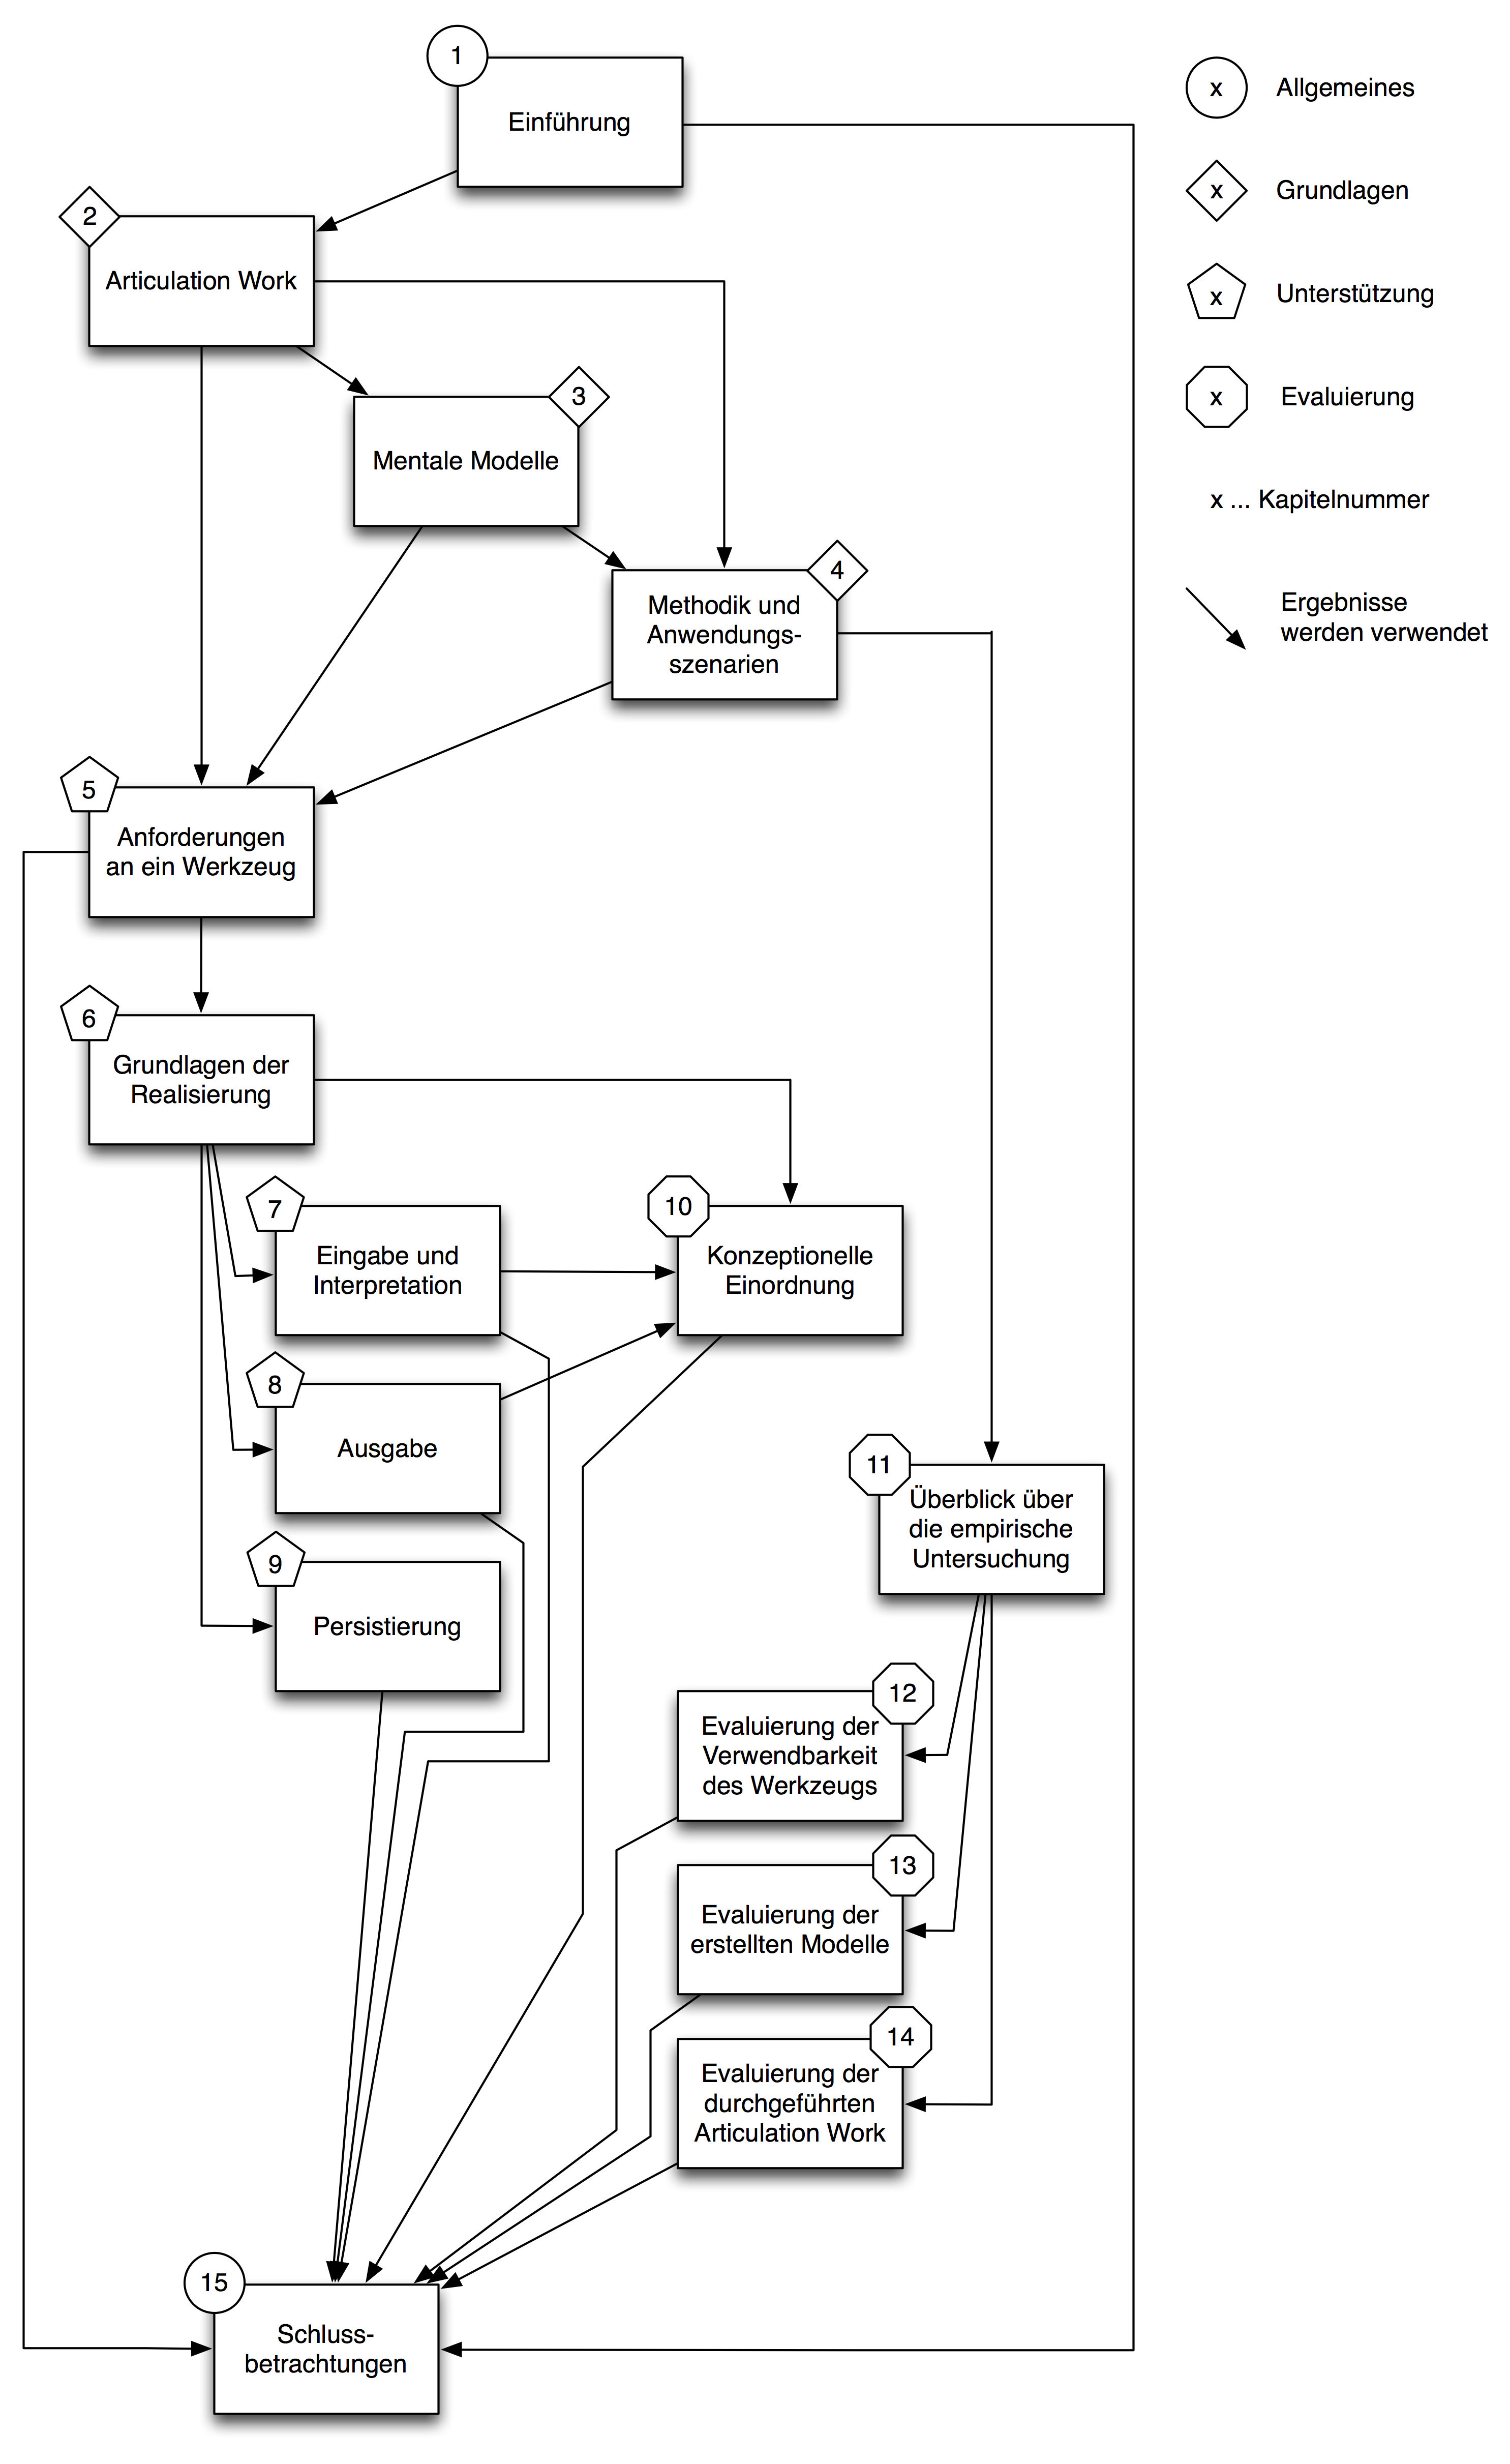
\includegraphics[scale=0.5]{img/Einfuehrung/gesamtueberblick.png}
	\caption{Zusammenhänge zwischen den Kapiteln der Arbeit}
	\label{fig:img_Einfuehrung_gesamtueberblick}
\end{figure}


% subsection zusammenhänge (end)
% section aufbau_der_arbeit (end)
